%%%%%%%%%%%%%%%%%%%%%%%%%%%%%%%%%%%%%%%%%%%%%%%%%%%%%%%%%%%%%%%%%%%%%%%%%%%%%%%%%%%%
%Do not alter this block of commands.  If you're proficient at LaTeX, you may include additional packages, create macros, etc. immediately below this block of commands, but make sure to NOT alter the header, margin, and comment settings here. 
\documentclass[12pt]{article}
 \usepackage[margin=1in]{geometry} 
\usepackage{amsmath,amsthm,amssymb,amsfonts, enumitem, fancyhdr, color, hyperref,comment, graphicx, environ,mathtools, bbm, tikz, setspace, cleveref,listings, dcolumn}
\usepackage{array, multirow, caption, booktabs}
\usepackage{lscape}
\usepackage{ mathrsfs }
\usetikzlibrary{matrix,positioning}
\tikzset{bullet/.style={circle,draw=black,inner sep=8pt}}
\DeclareMathOperator*{\argmax}{arg\,max}
\DeclareMathOperator*{\argmin}{arg\,min}
\DeclareMathOperator*{\Var}{\text{Var}}
\DeclareMathOperator*{\Cov}{\text{Cov}}

\DeclarePairedDelimiter\norm{\lVert}{\rVert}%
\newtheorem{theorem}{Theorem}
\newtheorem{lemma}[theorem]{Lemma}
\DeclareMathOperator{\eps}{\varepsilon}
\doublespacing
\DeclarePairedDelimiter\abs{\lvert}{\rvert}%
\pagestyle{fancy}
\setlength{\headheight}{65pt}
\newenvironment{problem}[2][Problem]{\begin{trivlist}
\item[\hskip \labelsep {\bfseries #1}\hskip \labelsep {\bfseries #2.}]}{\end{trivlist}}
\newenvironment{sol}
    {\emph{Solution:}
    }
    {
    \qed
    }


%%%%%%%%%%%%%%%%%%%%%%%%%%%%%%%%%%%%%%%%%%%%%%%%%%%%%%%%%%%%%%%%%%%%%%%%%%%%%%%%%


\usepackage{xcolor}
 
 


%%%%%%%%%%%%%%%%%%%%%%%%%%%%%%%%%%%%%%%%%%%%%

\rhead{Asha Bharadwaj, Caitlin Dutta, John Higgins, Alexis Smith\\Econ 899 \\ 6 December, 2022} 

%%%%%%%%%%%%%%%%%%%%%%%%%%%%%%%%%%%%%%%%%%%%


%%%%%%%%%%%%%%%%%%%%%%%%%%%%%%%%%%%%%%

\begin{document}
Note: the transition matrix $\Pi = \begin{bmatrix} 0.9 & 0.1\\ 0.9 & 0.1\end{bmatrix}$ given in the problem set differs from the transition matrix used to generate the supplied transition matrices as well as the simulated data (the transition matrix used for these appears to be $\Pi = \begin{bmatrix} 0.75 & 0.25\\0.9 & 0.1\end{bmatrix}$). We have proceeded using $\Pi = \begin{bmatrix} 0.75 & 0.25\\0.9 & 0.1\end{bmatrix}$ in our analysis for consistency).

\begin{problem}{1}
\end{problem}
\begin{sol}
    The implicit equation which defines $\bar{V}(s) = E_{\eps}[V(s, \eps)]$ is given by the following:
    \[\bar{V}(s) = \log(\exp(U_0(s)) + \exp(U_1(s))) + \gamma \]
    where $\gamma$ is Euler's constant and 
    \[U_0(s) = (\alpha c)\mathbbm{1}_{ i > 0} + \lambda \mathbbm{1}(i = 0, c > 0) \]
    \[U_1(s) = \alpha c - p\]
    with $s = (i, c, p)$ indicating the state.

    We solve for $\bar{V}(s)$ and tabulate the results in Table I for each state variable $s$. 
    \begin{table}
        \centering
        \begin{tabular}{|c|c|c|c|}
            \hline
            Inventory & Cons. shock & Price & $\bar{V}(s)$\\
            \hline 
            0.0 & 0.0 & 4.0 & 61.128 \\
            1.0 & 0.0 & 4.0 & 65.01 \\
            2.0 & 0.0 & 4.0 & 68.482 \\
            3.0 & 0.0 & 4.0 & 71.669 \\
            4.0 & 0.0 & 4.0 & 74.63 \\
            5.0 & 0.0 & 4.0 & 77.394 \\
            6.0 & 0.0 & 4.0 & 79.959 \\
            7.0 & 0.0 & 4.0 & 82.263 \\
            8.0 & 0.0 & 4.0 & 84.073 \\
            0.0 & 1.0 & 4.0 & 58.491 \\
            1.0 & 1.0 & 4.0 & 63.128 \\
            2.0 & 1.0 & 4.0 & 67.01 \\
            3.0 & 1.0 & 4.0 & 70.482 \\
            4.0 & 1.0 & 4.0 & 73.669 \\
            5.0 & 1.0 & 4.0 & 76.63 \\
            6.0 & 1.0 & 4.0 & 79.394 \\
            7.0 & 1.0 & 4.0 & 81.959 \\
            8.0 & 1.0 & 4.0 & 84.263 \\
            0.0 & 0.0 & 1.0 & 63.244 \\
            1.0 & 0.0 & 1.0 & 66.895 \\
            2.0 & 0.0 & 1.0 & 70.203 \\
            3.0 & 0.0 & 1.0 & 73.26 \\
            4.0 & 0.0 & 1.0 & 76.11 \\
            5.0 & 0.0 & 1.0 & 78.766 \\
            6.0 & 0.0 & 1.0 & 81.201 \\
            7.0 & 0.0 & 1.0 & 83.282 \\
            8.0 & 0.0 & 1.0 & 84.278 \\
            0.0 & 1.0 & 1.0 & 61.025 \\
            1.0 & 1.0 & 1.0 & 65.244 \\
            2.0 & 1.0 & 1.0 & 68.895 \\
            3.0 & 1.0 & 1.0 & 72.203 \\
            4.0 & 1.0 & 1.0 & 75.26 \\
            5.0 & 1.0 & 1.0 & 78.11 \\
            6.0 & 1.0 & 1.0 & 80.766 \\
            7.0 & 1.0 & 1.0 & 83.201 \\
            8.0 & 1.0 & 1.0 & 85.282 \\
            \hline
        \end{tabular}
        \caption{Values of $\bar{V}(s)$}
    \end{table}
\end{sol}
\begin{problem}{2}
\end{problem}

\begin{sol}
    We estimate the conditional choice probability $\hat{P}(s)$ using the provided simulated sequence of choices. Using this estimated $\hat{P}(s)$, we can compute the implied expected value function $\bar{V}^{\hat{P}}(s)$ using the CCP mapping. 

    Under the assumption that $\varepsilon \sim $ T1EV, it follows that $e(a, s) = \gamma - \ln(\hat{P}(s))$, where $e(a, s) = E[\eps(a) \mid a^* = a, s]$ is the conditional expectation of $\eps(a)$. The value function implied by the CCP vector is the following:
    \[\bar{V}^P = (I - \beta F^P)^{-1}[(1-P(s)) \odot (U_0(s) + e(0)) + P \odot (U_1(s) + e(1))]\]
    where $F^P = (1 - P) \odot F(0) + P \odot F(1)$ and $\odot$ is the Hadamard element-wise product operator.

    We first do one iteration of this operator using the estimated probabilities $\hat{P}$ to estimate $\bar{V}^{\hat{P}}(s)$ (i.e. one iteration of the above operator) and include our results in Table II. We see that they do differ from $\bar{V}(s)$, but only slightly (and not by very much on average). This could certainly be due to simulation error: some states are very unlikely to be realized in the sample, and we consequently will have fewer observations for those. This will adversely affect the accuracy of our implied value function estimate. We plot $\bar{V}(s)$ and $\bar{V}^{\hat{P}}(s)$ alongside each other in the following figure: 
    \begin{center}
        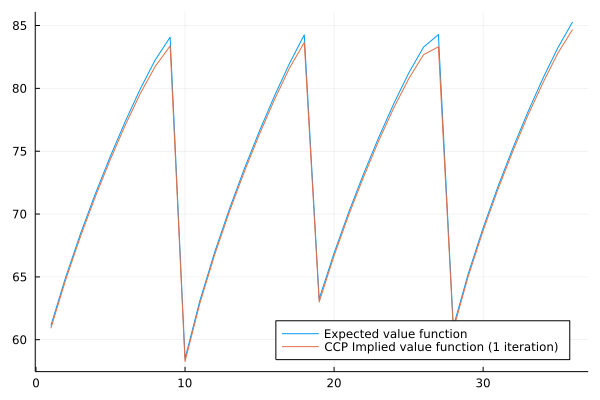
\includegraphics[scale=0.5]{vfplot.png}
    \end{center}
    We see that the only major differences occur for the states with very high $i$. These are extremely unlikely to be observed (as it is costly to build up that much inventory + consumption shocks will make it even harder to get that much). These are states for which the estimated $\hat{P} = 0.001$ (our imposed non-zero constraint). As a result, we shouldn't be surprised that the implied value function is a bit off.
   

    We have also iterated the CCP mapping (i.e. policy function iteration) to estimate $\bar{V}^{P}$. We iterate by updating $P^k = 1/(1 + \exp(- \tilde{v}(s)^{k-1}))$, where $\tilde{v}(s)^{k-1} = (U_1 + \beta F_1 \bar{V}^{k-1}) - (U_0 + \beta F(0) \bar{V}^{k-1})$. We stop when $\norm{P^k - P^{k-1}} < \eta$ (we use $\eta = 1 \times 10^{-12}$). When we iterate this until convergence, we get an estimate for $\bar{V}^{\hat{P}}(s)$ which is (not surprisingly) numerically identical to $\bar{V}(s)$ estimated in problem 1. We don't include the plot for this one because they're literally on top of each other and no information is gained that isn't conveyed in the table.
    \begin{table}
        \centering
        \begin{tabular}{|c|c|c|c|c|c|}
            \hline
            Inventory & Cons. shock & Price & $\bar{V}(s)$ & $\bar{V}^{\hat{P}}(s)$ (1 iter)& $\bar{V}^{P}(s)$ (actual) \\
            \hline 
    0.0 & 0.0 & 4.0 & 61.128 & 60.914 & 61.128 \\
    1.0 & 0.0 & 4.0 & 65.01 & 64.8 & 65.01 \\
    2.0 & 0.0 & 4.0 & 68.482 & 68.267 & 68.482 \\
    3.0 & 0.0 & 4.0 & 71.669 & 71.44 & 71.669 \\
    4.0 & 0.0 & 4.0 & 74.63 & 74.38 & 74.63 \\
    5.0 & 0.0 & 4.0 & 77.394 & 77.104 & 77.394 \\
    6.0 & 0.0 & 4.0 & 79.959 & 79.594 & 79.959 \\
    7.0 & 0.0 & 4.0 & 82.263 & 81.744 & 82.263 \\
    8.0 & 0.0 & 4.0 & 84.073 & 83.376 & 84.073 \\
    0.0 & 1.0 & 4.0 & 58.491 & 58.273 & 58.491 \\
    1.0 & 1.0 & 4.0 & 63.128 & 62.915 & 63.128 \\
    2.0 & 1.0 & 4.0 & 67.01 & 66.8 & 67.01 \\
    3.0 & 1.0 & 4.0 & 70.482 & 70.267 & 70.482 \\
    4.0 & 1.0 & 4.0 & 73.669 & 73.434 & 73.669 \\
    5.0 & 1.0 & 4.0 & 76.63 & 76.377 & 76.63 \\
    6.0 & 1.0 & 4.0 & 79.394 & 79.103 & 79.394 \\
    7.0 & 1.0 & 4.0 & 81.959 & 81.595 & 81.959 \\
    8.0 & 1.0 & 4.0 & 84.263 & 83.645 & 84.263 \\
    0.0 & 0.0 & 1.0 & 63.244 & 62.999 & 63.244 \\
    1.0 & 0.0 & 1.0 & 66.895 & 66.684 & 66.895 \\
    2.0 & 0.0 & 1.0 & 70.203 & 69.982 & 70.203 \\
    3.0 & 0.0 & 1.0 & 73.26 & 73.014 & 73.26 \\
    4.0 & 0.0 & 1.0 & 76.11 & 75.842 & 76.11 \\
    5.0 & 0.0 & 1.0 & 78.766 & 78.437 & 78.766 \\
    6.0 & 0.0 & 1.0 & 81.201 & 80.744 & 81.201 \\
    7.0 & 0.0 & 1.0 & 83.282 & 82.68 & 83.282 \\
    8.0 & 0.0 & 1.0 & 84.278 & 83.308 & 84.278 \\
    0.0 & 1.0 & 1.0 & 61.025 & 60.807 & 61.025 \\
    1.0 & 1.0 & 1.0 & 65.244 & 65.034 & 65.244 \\
    2.0 & 1.0 & 1.0 & 68.895 & 68.681 & 68.895 \\
    3.0 & 1.0 & 1.0 & 72.203 & 71.983 & 72.203 \\
    4.0 & 1.0 & 1.0 & 75.26 & 75.019 & 75.26 \\
    5.0 & 1.0 & 1.0 & 78.11 & 77.838 & 78.11 \\
    6.0 & 1.0 & 1.0 & 80.766 & 80.405 & 80.766 \\
    7.0 & 1.0 & 1.0 & 83.201 & 82.771 & 83.201 \\
    8.0 & 1.0 & 1.0 & 85.282 & 84.682 & 85.282 \\
    \hline
\end{tabular}
\caption{Values of $\bar{V}^{\hat{P}}(s)$ and true $\bar{V}^{P}(s)}
\end{table}
\end{sol}
\begin{problem}{3}
\end{problem}
\begin{sol}
   The log-likelihood function is given by the following:
   \[L(\lambda) = \sum_{i} a_i \ln(P(s_i)) + (1 - a_i) \ln(1 - P(s_i))\]
   such that $P(s_i) = \Psi(s_i) \equiv (1 + \exp(-\tilde{v}(s_i)^{k-1}))^{-1}$, where $\tilde{v}(s_i)^{k-1}$ is as defined previously.
\end{sol}
\begin{problem}{4}
\end{problem}
\begin{sol}
   We minimize the log-likelihood using the Nested-Fixed Point algorithm and find that the minimizer is $\hat{\lambda} = -4.024$, which corresponds to a log likelihood of -2633.152. We include a plot of the log-likelihood from $\lambda = -10$ to $\lambda = 0$ below:
   \begin{center}
    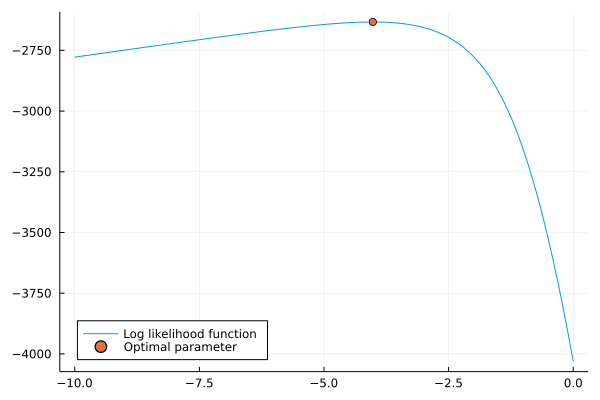
\includegraphics[scale=0.5]{llopt.png}
   \end{center}
\end{sol}
\end{document}